\documentclass[twoside]{article}
\setlength{\oddsidemargin}{0.25 in}
\setlength{\evensidemargin}{-0.25 in}
\setlength{\topmargin}{-0.6 in}
\setlength{\textwidth}{6.5 in}
\setlength{\textheight}{8.5 in}
\setlength{\headsep}{0.75 in}
\setlength{\parindent}{0 in}
\setlength{\parskip}{0.1 in}

%
% ADD PACKAGES here:
%
\usepackage{amsmath,amsfonts,graphicx,tikz}
\usepackage[most]{tcolorbox}
\usepackage[colorlinks=true, linkcolor=red, urlcolor=blue]{hyperref}
\usepackage{bbm}
\usetikzlibrary{calc,arrows.meta,decorations.pathreplacing}


\def\x0{0.6}
\pgfmathsetmacro{\ymax}{sqrt(1-(\x0)^2)}

\DeclareSymbolFont{extraup}{U}{zavm}{m}{n}
\DeclareMathSymbol{\varheart}{\mathalpha}{extraup}{86}
\DeclareMathSymbol{\vardiamond}{\mathalpha}{extraup}{87}

%
% The following commands set up the lecnum (lecture number)
% counter and make various numbering schemes work relative
% to the lecture number.
%
\newcounter{lecnum}
\renewcommand{\thepage}{\thelecnum-\arabic{page}}
\renewcommand{\thesection}{\thelecnum.\arabic{section}}
\renewcommand{\theequation}{\thelecnum.\arabic{equation}}
\renewcommand{\thefigure}{\thelecnum.\arabic{figure}}
\renewcommand{\thetable}{\thelecnum.\arabic{table}}

%
% The following macro is used to generate the header.
%
\newcommand{\lecture}[4]{
   \pagestyle{myheadings}
   \thispagestyle{plain}
   \newpage
   \setcounter{lecnum}{#1}
   \setcounter{page}{1}
   \noindent
   \begin{center}
   \framebox{
      \vbox{\vspace{2mm}
    \hbox to 6.28in { {\bf STAT 512: Statistical Inference
	\hfill Autumn 2025} }
       \vspace{4mm}
       \hbox to 6.28in { {\Large \hfill Lecture #1: #2  \hfill} }
       \vspace{2mm}
       \hbox to 6.28in { {\it Instructor: #3 \hfill Tony Lei} }
      \vspace{2mm}}
   }
   \end{center}
   \markboth{Lecture #1: #2}{Lecture #1: #2}

   \vspace*{4mm}
}

%for the motivation box
\tcbset{
  motivationstyle/.style={
    colback=gray!10!white,   % light gray background
    colframe=gray!70!black,  % darker gray border
    fonttitle=\bfseries,
    title=Motivation,
    sharp corners,
    boxrule=0.8pt,
    coltitle=black,
    enhanced
  }
}

\newenvironment{motivation}
  {\begin{tcolorbox}[motivationstyle]}
  {\end{tcolorbox}}

%Use this command for a figure
\newcommand{\fig}[3]{
			\vspace{#2}
			\begin{center}
			Figure \thelecnum.#1:~#3
			\end{center}
	}

% Red note command
\newcommand{\note}[1]{\textcolor{red}{#1}}

% Use these for theorems, lemmas, proofs, etc.
\newtheorem{theorem}{Theorem}[lecnum]
\newtheorem{lemma}[theorem]{Lemma}
\newtheorem{proposition}[theorem]{Proposition}
\newtheorem{claim}[theorem]{Claim}
\newtheorem{question}[theorem]{Question}
\newtheorem{answer}[theorem]{Answer}
\newtheorem{corollary}[theorem]{Corollary}
\newtheorem{definition}[theorem]{Definition}
\newenvironment{proof}{{\bf Proof:}}{\hfill\rule{2mm}{2mm}}

% **** ADDITIONAL MACROS:
\newcommand\E{\mathbb{E}}
\newcommand\F{\mathcal{F}}
\newcommand{\prob}{\mathbb{P}}

\begin{document}
\lecture{2}{Transforming continuous random variables}{Ema Perkovic}
Suppose that we have a random variable $X$, desnity function $p_X(x)$ and a measurable function $g$. Then now suppose we define a new random variable $Y$ to be 
$$
g(X)=Y
$$
The natural question is to ask: What is the distribution of $Y$?

\section{One function of one random variable}

Let $X$ be a continuous random variable whose PDF $p_X(x)$ is known.
Consider a given function $f$ and another random variable $Y = g(X)$. 
Since the input $X$ is random, the output $Y$ is often random as well. 
What will the distribution of $Y$ be?

When $f$ is differentiable, we have the following useful theorem.

\begin{theorem}
In the above setting and assume that $X\in[a,b]$  and $g'(x)>0$ (strictly increasing) over $[a,b]$, then the PDF of $Y$
$$
p_Y(y) = \begin{cases}
\frac{p_X(f^{-1}(y))}{f'(f^{-1}(y))},\quad &f(a)\leq y\leq f(b)\\
0,\quad&\mbox{otherwise}.
\end{cases}
$$
\label{thm::simple}
\end{theorem}
\begin{proof}

To start with, we consider the CDF of $Y$:
\begin{align*}
P(Y\leq y) & = P(f(X)\leq y)\\
& = P(X\leq f^{-1}(y)).
\end{align*}
The PDF will be the derivative of the CDF, leading to 
\begin{align*}
p_Y(y) & = \frac{d}{dy} P(Y\leq y)\\
& = \frac{d}{dy}P(X\leq f^{-1}(y))\\
& = p_X(f^{-1}(y)) \frac{d}{dy} f^{-1}(y)\\
& = \frac{p_X(f^{-1}(y))}{f'(f^{-1}(y))},
\end{align*}
which completes the proof.
\end{proof}

{\bf Example.}
Suppose $f(x) = x^2$ and $X\sim {\sf Uniform}[0,1]$. 
And we are interested in the PDF of $Y = f(X)  = X^2$. 
Because $f'(x) = 2x$ and $X\geq 0$ so $f^{-1}(y) = \sqrt{y}$,
we have
\begin{align*}
p_Y(y) = \frac{1}{2\sqrt{y}}I(0\leq y\leq 1).
\end{align*}

{\bf Example.}
Assume $X\sim {\sf Uniform}[0,1]$ and consider $f(x) = -2\log X$
and let $Y = -2\log X$. 
In this case, $f'(x)  = -\frac{2}{X}$ and $f^{-1}(y) = e^{-\frac{1}{2}y}$.
However, $f'(x)$ is negative so we cannot directly apply Theorem~\ref{thm::simple}.
A simple modification shows that the same formula holds as long as we replace $f'(f^{-1}(y))$
by $|f'(f^{-1}(y))|$ (think about why).

Then the PDF of $Y$ will be 
\begin{align*}
p_Y(y) = \frac{1}{2}e^{-\frac{1}{2}y}I(0\leq y)
\end{align*}
which is the Exponential distribution with parameter $\lambda = \frac{1}{2}$.
 
{\bf Example.}
Suppose that $Y$ is a continuous random variable with CDF $F_Y$
and $X$ is a uniform random variable within $[0,1]$. 
Then you can show that $Z = F_Y^{-1}(X)$ has a CDF $F_Z(z) = F_Y(z)$.
More generally, we have 
\begin{theorem}
    Let $X$ be a continious random variable with PDF, $P_X(x)$. Let $g:\mathbb{R}\rightarrow\mathbb{R}$ be differentialable and strictly monotonic function with inverse $\gamma = g^{-1}$. Then the PDF of $y=g(x)$ is given by $$p_Y(y)= \begin{cases}\left|\gamma^{\prime}(y)\right| p_X\left(g^{-1}(y)\right) & y \in g(\mathbb{R}) \\ 0 & \text { otherwise }\end{cases}$$
\end{theorem}
\begin{proof}
Denote $a=\inf _x(g(x)), b=\sup _x(g(x))$, (possibly $a=-\infty$, or $b=+\infty$ ) If $t<a, F_Y(t)=P(g(X) \leq a)=0$ so $p_Y(t)=0$. If $t>b, F_Y(t)=P(g(X) \leq t)=1$ so $p_Y(t)=0$.
If $g$ is strictly increasing, for $t \in(a, b)$, then $\gamma(t):=g^{-1}(t)$ is defined,

$$
\begin{aligned}
F_Y(t) & =P(Y \leq t)=P(g(X) \leq t)=P\left(X \leq g^{-1}(t)\right)=F_X(\gamma(t)) \\
\text { so } \quad p_Y(t) & =\gamma^{\prime}(t) p_X(\gamma(t))
\end{aligned}
$$


If $g$ is strictly decreasing, for $t \in(a, b)$, then $g^{-1}(t)$ is defined,

$$
\begin{aligned}
F_Y(t) & =P(Y \leq t)=P(g(X) \leq t)=P\left(X \geq g^{-1}(t)\right)=1-F_X(\gamma(t)) \\
\text { so } \quad p_Y(t) & =-\gamma^{\prime}(t) p_X(\gamma(t))
\end{aligned}
$$


For $t \in(a, b), g \circ g^{-1}(t)=t$ so $\gamma^{\prime}(t)=\frac{1}{g^{\prime}\left(g^{-1}(t)\right)}$ so $\gamma^{\prime}(t)<0$ for $g$ decreasing.\newline
\note{If $g$ is not defined on $\mathbb{R}$ but rather, $g:B\rightarrow\mathbb{R}$ for some $B\subseteq\mathbb{R}$, we can still use the above theorem as long as $P(X\in B)=1$} 
\end{proof}

{\bf Example.}
Assume $X\sim {\sf Uniform}[1,e]$ and consider that we are interested in the PDF of $Y$ where $Y=-2\ln X$. Here $g(x)=-2\ln(x), x\in [1,e]$. Then, $g'(x)=\frac{-2}{x}$, so $g'(x)<0, x\in [1,e]$ which is strictly decreasing.

We also have that when $x=1,-2\ln(1)=0$ and $-2\ln(e)=-2$. Hence the range of $g(x)$ is $[-2,0]$

The PDF of $X$ is given as $p_X(x)=\frac{1}{e-1}$ and $g^{-1}(y)=e^{-\frac{1}{2}}(x)$. Thus, by Theorem 2.2, we have
$$
p_Y(y)=\frac{1}{2(e-1)}e^{-\frac{1}{2}y}\mathbbm{1}
$$

Now, what if the $g(x)$ is not strictly monotone over the entire domain? In this case, we will split the domain over where it is monotonic and then use the law of total probability. 

{\bf Example.}
Consider $X\sim N(0,1)$ and $Y =  X^2$.
What is the distribution of $Y$?
Note that the underlying transformation $f(x) =x^2$ 
is not always increasing or decreasing since $x\in\mathbb{R}$.
In this case, a general strategy is to work out the CDF:
\begin{align*}
F_Y(y) &= P(Y\leq y)\\
& = P(X^2\leq y) \\
& = P(-\sqrt{y}\leq X\leq \sqrt{y})\\
&  = F_X(\sqrt{y})-F_X(-\sqrt{y}).
\end{align*}
Thus,
\begin{align*}
p_Y(y) &= \frac{d}{dy}[F_X(\sqrt{y})-F_X(-\sqrt{y})]\\
& = \frac{1}{2\sqrt{y}}(p_X(\sqrt{y}) + p_X(-\sqrt{y})).
\end{align*}
In this case, because $X\sim N(0,1)$, it is symmetric so we further have 
$$
p_Y(y) = \frac{1}{\sqrt{y}}p_X(\sqrt{y}).
$$
Putting $p_X(x) = \frac{1}{\sqrt{2\pi}}e^{-x^2/2}$ into the above equation, we obtain
$$
p_Y(y) = \frac{1}{\sqrt{y}}\frac{1}{\sqrt{2\pi}}e^{-y/2} = \frac{1}{\sqrt{2\pi}}y^{-\frac{1}{2}}e^{-\frac{1}{2}y},
$$
which is Gamma $(\frac{1}{2},\frac{1}{2})$.
Note: Gamma $(\frac{1}{2},\frac{1}{2})$ is the same as $\chi^2_1$, the chi-squared distribution with degree of freedom $1$. 
\note{If $X$ comes from a standard normal, then the square of a standard normal is a $\chi^2$ with df=$1$.}
\section{One function of two or more random variables}

In practice, we may encounter problems involving a function of two or more random variables. 
Namely, we have $X,Y$ two random variables whose joint distribution $p(x,y)$ is known
and we are interested in the distribution of another random variable $U = f(X,Y)$ for some given function $f$.
In this case, a general strategy is to investigate the underlying CDF and take the derivative to obtain the corresponding PDF. 
Here we will illustrate the idea via a few examples. 

\begin{itemize}
\item {\bf Case 1: $U= X+Y$.}
{\bf Example (Sum of Uniform)}
Consider $X,Y$ random variables which are both iid $\sim$ Uniform$[0,1]$. What is the distribution of $X+Y=U?$
The domain is given by $0\leq X+Y\leq 2$. Visually, we have that 
$$p_{x,y}(x,y)=1$$ for each point in the unit square since they are independent. 
\begin{center}
\resizebox{\textwidth}{!}{%
\begin{tikzpicture}[>=stealth]

% ---------- parameters ----------
\def\uA{0.65}  % left panel u in (0,1)
\def\uB{1.55}  % right panel u in (1,2)

% -------- LEFT: 0<u<1 --------
\begin{scope}[scale=4.2]
  % axes and unit square
  \draw[->] (-0.02,0) -- (1.15,0) node[right] {$x$};
  \draw[->] (0,-0.02) -- (0,1.15) node[above] {$y$};
  \draw[thick] (0,0) rectangle (1,1);
  \draw (1,0) -- ++(0,0.02) node[below=2pt] {$1$};
  \draw (0,1) -- ++(0.02,0) node[left=2pt] {$1$};
  \node[below left] at (0,0) {$0$};

  % guide lines
  \draw[gray!80] (0,1) -- (1,0) node[pos=.55,below right=-2pt] {$x+y=1$};

  % x+y = u and shaded triangle
  \draw[thick] (0,\uA) -- (\uA,0);
  \node at (0.65,0.25) {$x+y=\uA$};

  \begin{scope}
    \clip (0,0) rectangle (1,1);
    \fill[black!60,opacity=.25] (0,0) -- (\uA,0) -- (0,\uA) -- cycle;
    \draw[black!60] (0,0) -- (\uA,0) -- (0,\uA) -- cycle;
  \end{scope}

  % braces
  \draw[decorate,decoration={brace,mirror,raise=2pt}] (0,0) -- (\uA,0)
        node[midway,below=4pt] {$u$};
  \draw[decorate,decoration={brace,raise=2pt}] (0,0) -- (0,\uA)
        node[midway,left=4pt] {$u$};

  % caption
  \node at (0.8,-0.20) {$\{(x,y)\in[0,1]^2:\ x+y\le u\},\ 0<u<1$};
\end{scope}

% -------- RIGHT: 1<u<2 --------
\begin{scope}[xshift=8.5cm,scale=4.2] % shift enough; resizebox will fit it all
  % axes and unit square
  \draw[->] (-0.02,0) -- (1.15,0) node[right] {$x$};
  \draw[->] (0,-0.02) -- (0,1.15) node[above] {$y$};
  \draw[thick] (0,0) rectangle (1,1);
  \draw (1,0) -- ++(0,0.02) node[below=2pt] {$1$};
  \draw (0,1) -- ++(0.02,0) node[left=2pt] {$1$};
  \node[below left] at (0,0) {$0$};

  % line x+y=u
  \coordinate (A) at ({\uB-1},1);
  \coordinate (B) at (1,{\uB-1});
  \draw[thick] (0,\uB) -- (\uB,0);
  \node at (0.6,1.3) {$x+y=\uB$};

  % shaded region: square minus top-right triangle
  \begin{scope}
    \clip (0,0) rectangle (1,1);
    \fill[black!60,opacity=.25] (0,0) rectangle (1,1);
    \fill[white] (A) -- (1,1) -- (B) -- cycle;
    \draw[black!60] (A) -- (1,1) -- (B) -- cycle;
  \end{scope}

  % braces (optional)
  \draw[decorate,decoration={brace,raise=2pt}] (A) -- (1,1)
        node[midway,above=3pt] {$2-\uB$};
  \draw[decorate,decoration={brace,mirror,raise=2pt}] (1,{\uB-1}) -- (1,0)
        node[midway,right=3pt] {$2-\uB$};

  % caption
  \node at (0.8,-0.20) {$\{(x,y)\in[0,1]^2:\ x+y\le u\},\ 1<u<2$};
\end{scope}

\end{tikzpicture}%
}% end resizebox
\end{center}

\begin{align*}
    F_U(u) &= \prob(U\leq u)= \prob(X+Y\leq u)\\
\end{align*}
Visually, we can calculate the area of the region in the unit square to be 
\[
\begin{cases}
    0 & u<0\\
    \frac{u^2}{2} & 0\leq u \leq 1\\
    1-\frac{(2-u)^2}{2} & 1\leq u \leq 2\\
    1 & u\geq 2
\end{cases}
\]

The pdf is then given by
\[
\begin{cases}
    0 & u<0\\
    u & 0\leq u < 1\\
    (2-u) & 1\leq u \leq 2\\
    0 & u\geq 2
\end{cases}
\]
\begin{proposition}
Let $X,Y$ be indepedent RV and let Z=X+Y. If $X$ and $Y$ are both conitnious, then the CDF of $Z$ can be computed as 
Then the CDF of $Z$ can be computed as:
\[
F_Z(z)=\Pr(Z\le z)=\Pr(X+Y\le z)
= \int_{-\infty}^{+\infty} F_X(z-t)\,p_Y(t)\,dt
= \int_{-\infty}^{+\infty} F_Y(z-t)\,p_X(t)\,dt .
\]

and the PDF of $Z$ can be computed as:
\[
p_Z(z)=\int_{-\infty}^{+\infty} p_X(z-t)\,p_Y(t)\,dt
= \int_{-\infty}^{+\infty} p_Y(z-t)\,p_X(t)\,dt .
\]

For discrete $X,Y$, we have the following expressions for the CDF and PMF of $Z$:
\[
F_Z(z)=\Pr(X+Y\le z)
= \sum_{k=-\infty}^{+\infty} F_X(z-k)\,p_Y(k)
= \sum_{k=-\infty}^{+\infty} F_Y(z-k)\,p_X(k),
\]
\[
p_Z(z)=\sum_{k=-\infty}^{+\infty} p_X(z-k)\,p_Y(k)
= \sum_{k=-\infty}^{+\infty} p_Y(z-k)\,p_X(k).
\]

Consider, using the above proposition to compute $p_U(u)$ directly for $u\in[0,2)$. We have that
\[
p_U(u)=\int_{-\infty}^{+\infty} p_X(u-t)\,p_Y(t)\,dt .
\]

\end{proposition}
\item {\bf Case 2: $U= \max\{X,Y\}$.}
A common trick to compute the distribution of a maximum of two or more independent random variables is based on the following insight:
$$
\{\max\{X,Y\}\leq u\} \equiv \{X\leq u,  Y\leq u\}.
$$
Therefore, 
$$
F_U(u) = P(U\leq u) = P(\max\{X,Y\}\leq u) = P(X\leq u, Y\leq u) = P(X\leq u)P(U\leq u),
$$
which implies $F_U(u) = u^2$ and $p_U(u) = 2u$
when $u\in[0,1]$.



\item {\bf Case 3: $U= \min\{X,Y\}$.}
The case of minimum is similar to the case of maximal but we will consider a reverse event:
$$
\{\min\{X,Y\}> u\} \equiv \{X> u,  Y> u\}.
$$
Therefore.
$$
1-F_U(u) = P(U> u) = P(\min\{X,Y\}> u) = P(X> u, Y> u) = P(X> u)P(U> u)  = (1-u)^2,
$$
Thus, $F_U(u) = 1-(1-u)^2$ so $p_U(u) = 2-2u$ for $u\in[0,1]$.

\end{itemize}




{\bf Example (minimum of many uniforms).}
Now consider $X_1,\cdots, X_n$ that are IID from a uniform distribution over $[0,1]$. 
Define $U = n \min\{X_1,\cdots, X_n\}$. 
What will the distribution of $U$ be when $n $ is large?
Using the trick that we have discussed, 
$$
\{\min\{X_1,\cdots,X_n\}> u\} \equiv \{X_1> u,\cdots,  X_n> u\},
$$
so 
$$
1-F_U(u) = P\left(\min\{X_1,\cdots,X_n\}> \frac{u}{n}\right) = \prod_{i=1}^n P\left(X_i>\frac{u}{n}\right) = \left(1-\frac{u}{n}\right)^n \rightarrow e^{-u}.
$$
As a result, $F_U(u) \rightarrow 1-e^{-u}$ and $p_U(u)\rightarrow e^{-u}$
so when $n$ is large, $U$ behaves like from an Exponential distribution. 





{\bf Example (exponential distributions).}
Consider $X,Y$ are IID from exponential distribution with parameter $1$. 
\begin{itemize}
\item {\bf Sum of two exponentials.} 
What is the distribution of $U = X+Y?$ 
A simple trick is to fixed one variable at a time and make good use of integration. 
Specifically, for a given $u>0$, 
\begin{align*}
F_U(u)&= P(U\leq u)\\
& = P(X+Y\leq u)\\
& = \int_{x+y\leq u} e^{-x-y}dxdy\\
& = \int_{x=0}^u \int_{y=0}^{u-x} e^{-x-y}dydx\\
& = \int_{x=0}^u e^{-x} (1-e^{x-u})dx\\
& = 1-e^{-u}-ue^{-u}.
\end{align*}
Thus, $p_U(u) = ue^{-u}$.


\item {\bf Minimum of two exponentials.} 
Now we consider $V = \min\{X,Y\}$. 
Using the same trick as the minimum of many uniforms, i.e.,
$$
\{\min\{X,Y\}>v\} \equiv \{X>v,Y>v\}
$$
so 
$$
1-F_V(v) = P(X>v)P(Y>v) = e^{-2v},
$$
which implies that $V\sim {\sf Exp}(2)$. 
In fact, you can easily generalize it to showing that if $X_1,\cdots, X_n\sim {\sf Exp}(\lambda)$,
then $\min\{X_1,\cdots, X_n\}\sim {\sf Exp}(n\lambda)$.


\item {\bf Difference.} 
Consider 
$$
Z = \max\{X,Y\} - \min\{X,Y\} = |X-Y|.
$$
What will the distribution of $Z$ be? 

Using a direct computation, we see that 
\begin{align*}
F_Z(z) & = P(Z\leq z)\\
& = P(|X-Y|\leq z)\\
& = P(-z\leq X-Y\leq z)\\
& = P(X- Y\leq z) - P(X-Y< -z)\\
& = P(X\leq Y+z) - 1+P(X-Y\geq -z)\\
& = -1 +P(X\leq Y+z) + P(Y\leq X+z)\\
&= -1 + 2P(X\leq Y+z) \qquad\mbox{$X,Y$ are symmetriic}.
\end{align*}
Moreover, 
\begin{align*}
P(X\leq Y+z) & = \int_{y=0}^\infty \int_{x=0}^{y+z} e^{-x}dx e^{-y}dy\\
& =  \int_{y=0}^\infty (1-e^{-y-z})e^{-y}dy\\
& = 1-e^{-z}\int_0^\infty e^{-2y}dy\\
& = 1-\frac{1}{2}e^{-z}.
\end{align*}
As a result,
$$
F_Z(z) = -1 + 2P(X\leq Y+z) = 1-e^{-z},
$$
which is the CDF of ${\sf Exp}(1)$!
This is another \emph{memoryless property}.


\item {\bf Ratio.} 
Finally, we consider 
$
W = \frac{X}{X+Y}
$
and studies its distribution.
Clearly, $0\leq w\leq 1$ so we will focus on the range $[0,1]$.
\begin{align*}
F_W(w) & = P\left(\frac{X}{X+Y}\leq w\right)\\
& = P(X\leq w(X+Y))\\
& = P((1-w)X\leq wY)\\
& = P\left(X\leq \frac{w}{1-w} Y\right)\\
& = \int_{y=0}^\infty \int_{x=0}^{\frac{w}{1-w}y}e^{-x}dx e^{-y}dy\\
& = \int_{y=0}^\infty (1-e^{\frac{-w}{1-w}y}) e^{-y}dy\\
& = 1 -\int_0^\infty e^{-\frac{1}{1-w}y}dy\\
& = 1- 1+w = w. 
\end{align*}
Thus $W\sim {\sf Unif}[0,1]$.

\end{itemize}



{\bf Useful properties about normal}
\begin{itemize}
\item Let $X\sim N(\mu_1,\sigma^2)$ and $Y\sim N(\mu_2,\sigma_2^2)$ be independent.
Then 
$$
X+Y \sim N(\mu_1+\mu_2, \sigma_1^2+\sigma_2^2)
$$
Also, for any real number $a$,
$$
aX \sim N(a\mu_1, a^2 \sigma_1^2).
$$

\item Let $X_1,\cdots, X_n$ be IID normal random variables from $N(\mu,\sigma^2)$.
Then the sample mean
$$
\bar X_n = \frac{1}{n}\sum_{i=1}^n X_i\sim N(\mu,\sigma^2/n).
$$

\item Let $X_1,\cdots, X_n$ be IID normal random variables from $N(0,1)$.
Then $Z_1 = X_1^2$ follows the $\chi^2$ distribution with a degree of freedom $1$.
And $Z_n = \sum_{i=1}^n X_i^2$ follows the  $\chi^2$ distribution with a degree of freedom $n$.

\end{itemize}



\end{document}